\documentclass{standalone}
\usepackage{tikz}
\usetikzlibrary{patterns, positioning}


\begin{document}
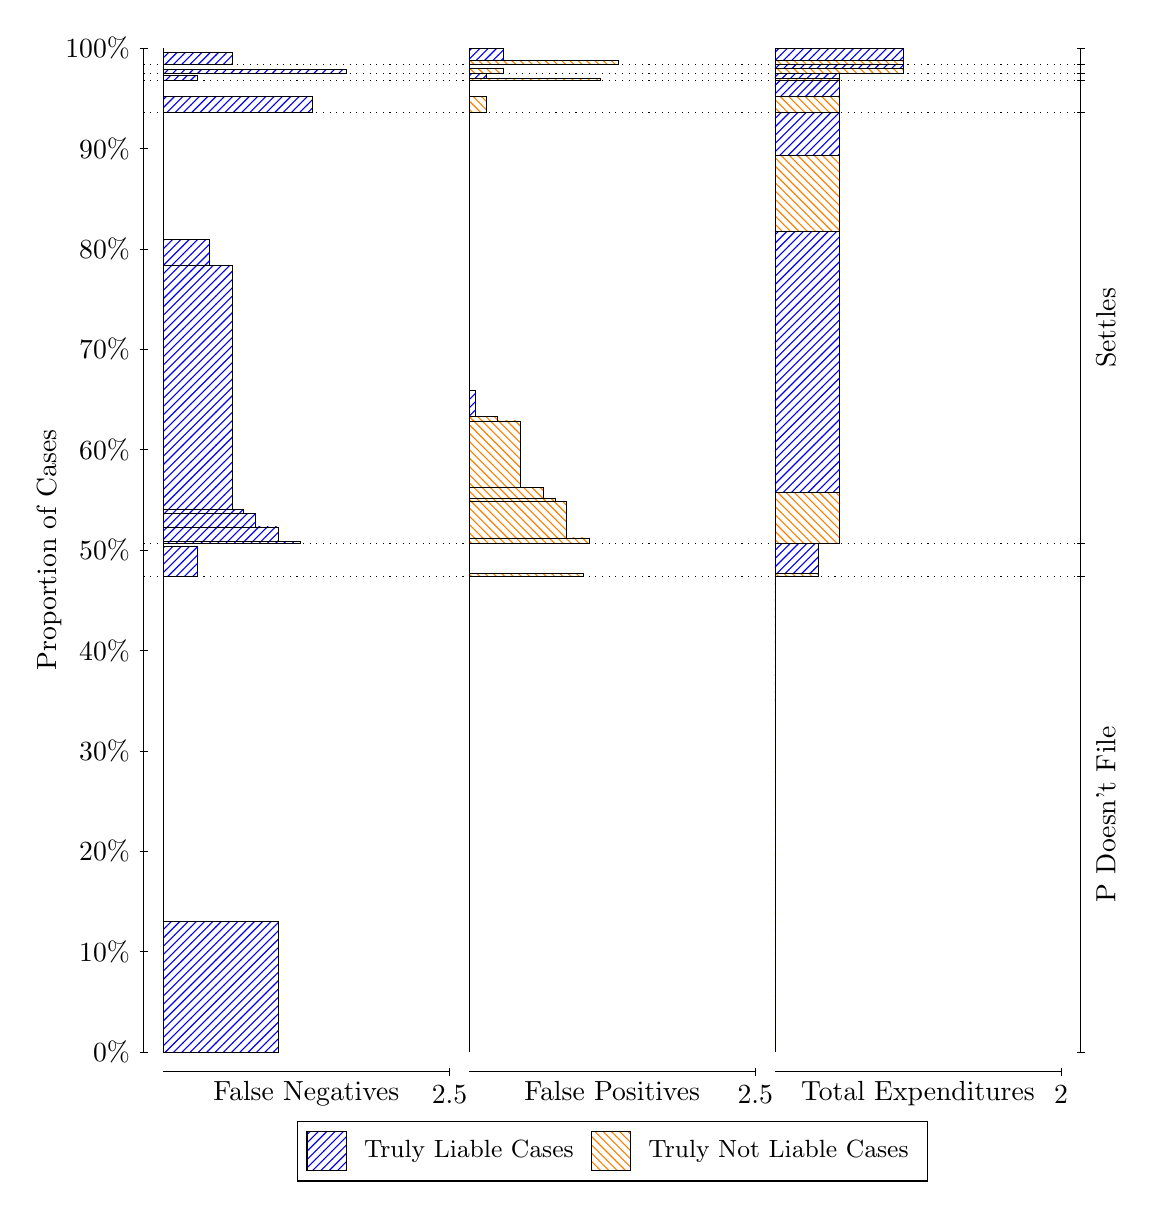
\begin{tikzpicture}
\draw[black, very thin] (1.5,1.75) -- (1.5,14.5);
\node[rotate=90, text=black, anchor=center] at (0.3, 8.125) {Proportion of Cases};
\draw[black, very thin] (1.45,1.75) -- (1.55,1.75);
\node[text=black, anchor=east] at (1.45, 1.75) {0\%};
\draw[black, very thin] (1.45,3.025) -- (1.55,3.025);
\node[text=black, anchor=east] at (1.45, 3.025) {10\%};
\draw[black, very thin] (1.45,4.3) -- (1.55,4.3);
\node[text=black, anchor=east] at (1.45, 4.3) {20\%};
\draw[black, very thin] (1.45,5.575) -- (1.55,5.575);
\node[text=black, anchor=east] at (1.45, 5.575) {30\%};
\draw[black, very thin] (1.45,6.85) -- (1.55,6.85);
\node[text=black, anchor=east] at (1.45, 6.85) {40\%};
\draw[black, very thin] (1.45,8.125) -- (1.55,8.125);
\node[text=black, anchor=east] at (1.45, 8.125) {50\%};
\draw[black, very thin] (1.45,9.4) -- (1.55,9.4);
\node[text=black, anchor=east] at (1.45, 9.4) {60\%};
\draw[black, very thin] (1.45,10.675) -- (1.55,10.675);
\node[text=black, anchor=east] at (1.45, 10.675) {70\%};
\draw[black, very thin] (1.45,11.95) -- (1.55,11.95);
\node[text=black, anchor=east] at (1.45, 11.95) {80\%};
\draw[black, very thin] (1.45,13.225) -- (1.55,13.225);
\node[text=black, anchor=east] at (1.45, 13.225) {90\%};
\draw[black, very thin] (1.45,14.5) -- (1.55,14.5);
\node[text=black, anchor=east] at (1.45, 14.5) {100\%};

\draw[black, very thin] (13.4,1.75) -- (13.4,14.5);
\draw[black, very thin] (13.35,1.75) -- (13.45,1.75);
\node[anchor=west] at (13.35, 1.75) {};
\draw[black, very thin] (13.35,7.7899) -- (13.45,7.7899);
\node[anchor=west] at (13.35, 7.7899) {};
\draw[black, very thin] (13.35,8.2111) -- (13.45,8.2111);
\node[anchor=west] at (13.35, 8.2111) {};
\draw[black, very thin] (13.35,13.68) -- (13.45,13.68);
\node[anchor=west] at (13.35, 13.68) {};
\draw[black, very thin] (13.35,14.088) -- (13.45,14.088);
\node[anchor=west] at (13.35, 14.088) {};
\draw[black, very thin] (13.35,14.174) -- (13.45,14.174);
\node[anchor=west] at (13.35, 14.174) {};
\draw[black, very thin] (13.35,14.29) -- (13.45,14.29);
\node[anchor=west] at (13.35, 14.29) {};
\draw[black, very thin] (13.35,14.5) -- (13.45,14.5);
\node[anchor=west] at (13.35, 14.5) {};

\draw[black, very thin, pattern color=blue, pattern=north east lines] (1.75,1.75) rectangle (3.2033,3.4071);
\draw[black, very thin, pattern color=orange, pattern=north west lines] (1.75,3.4071) rectangle (1.75,7.7899);
\draw[black, very thin, pattern color=blue, pattern=north east lines] (1.75,7.7899) rectangle (2.186,8.1692);
\draw[black, very thin, pattern color=orange, pattern=north west lines] (1.75,8.1692) rectangle (1.75,8.2111);
\draw[black, very thin, pattern color=blue, pattern=north east lines] (1.75,8.2111) rectangle (3.494,8.2362);
\draw[black, very thin, pattern color=blue, pattern=north east lines] (1.75,8.2362) rectangle (3.2033,8.4194);
\draw[black, very thin, pattern color=blue, pattern=north east lines] (1.75,8.4194) rectangle (2.9127,8.5893);
\draw[black, very thin, pattern color=blue, pattern=north east lines] (1.75,8.5893) rectangle (2.7673,8.6414);
\draw[black, very thin, pattern color=blue, pattern=north east lines] (1.75,8.6414) rectangle (2.622,11.738);
\draw[black, very thin, pattern color=blue, pattern=north east lines] (1.75,11.738) rectangle (2.3313,12.069);
\draw[black, very thin, pattern color=orange, pattern=north west lines] (1.75,12.069) rectangle (1.75,13.68);
\draw[black, very thin, pattern color=blue, pattern=north east lines] (1.75,13.68) rectangle (3.6393,13.887);
\draw[black, very thin, pattern color=orange, pattern=north west lines] (1.75,13.887) rectangle (1.75,14.088);
\draw[black, very thin, pattern color=blue, pattern=north east lines] (1.75,14.088) rectangle (2.186,14.152);
\draw[black, very thin, pattern color=orange, pattern=north west lines] (1.75,14.152) rectangle (1.75,14.174);
\draw[black, very thin, pattern color=blue, pattern=north east lines] (1.75,14.174) rectangle (4.0753,14.225);
\draw[black, very thin, pattern color=orange, pattern=north west lines] (1.75,14.225) rectangle (1.75,14.29);
\draw[black, very thin, pattern color=blue, pattern=north east lines] (1.75,14.29) rectangle (2.622,14.449);
\draw[black, very thin, pattern color=orange, pattern=north west lines] (1.75,14.449) rectangle (1.75,14.5);
\draw[black, very thin, pattern color=orange, pattern=north west lines] (5.6333,1.75) rectangle (5.6333,6.1328);
\draw[black, very thin, pattern color=blue, pattern=north east lines] (5.6333,6.1328) rectangle (5.6333,7.7899);
\draw[black, very thin, pattern color=orange, pattern=north west lines] (5.6333,7.7899) rectangle (7.0867,7.8318);
\draw[black, very thin, pattern color=blue, pattern=north east lines] (5.6333,7.8318) rectangle (5.6333,8.2111);
\draw[black, very thin, pattern color=orange, pattern=north west lines] (5.6333,8.2111) rectangle (7.1593,8.2785);
\draw[black, very thin, pattern color=orange, pattern=north west lines] (5.6333,8.2785) rectangle (6.8687,8.7459);
\draw[black, very thin, pattern color=orange, pattern=north west lines] (5.6333,8.7459) rectangle (6.7233,8.781);
\draw[black, very thin, pattern color=orange, pattern=north west lines] (5.6333,8.781) rectangle (6.578,8.9246);
\draw[black, very thin, pattern color=orange, pattern=north west lines] (5.6333,8.9246) rectangle (6.2873,9.7658);
\draw[black, very thin, pattern color=orange, pattern=north west lines] (5.6333,9.7658) rectangle (5.9967,9.8226);
\draw[black, very thin, pattern color=blue, pattern=north east lines] (5.6333,9.8226) rectangle (5.706,10.153);
\draw[black, very thin, pattern color=blue, pattern=north east lines] (5.6333,10.153) rectangle (5.6333,13.68);
\draw[black, very thin, pattern color=orange, pattern=north west lines] (5.6333,13.68) rectangle (5.8513,13.881);
\draw[black, very thin, pattern color=blue, pattern=north east lines] (5.6333,13.881) rectangle (5.6333,14.088);
\draw[black, very thin, pattern color=orange, pattern=north west lines] (5.6333,14.088) rectangle (7.3047,14.111);
\draw[black, very thin, pattern color=blue, pattern=north east lines] (5.6333,14.111) rectangle (5.8513,14.174);
\draw[black, very thin, pattern color=orange, pattern=north west lines] (5.6333,14.174) rectangle (6.0693,14.239);
\draw[black, very thin, pattern color=blue, pattern=north east lines] (5.6333,14.239) rectangle (5.6333,14.29);
\draw[black, very thin, pattern color=orange, pattern=north west lines] (5.6333,14.29) rectangle (7.5227,14.341);
\draw[black, very thin, pattern color=blue, pattern=north east lines] (5.6333,14.341) rectangle (6.0693,14.5);
\draw[black, very thin, pattern color=orange, pattern=north west lines] (9.5167,1.75) rectangle (9.5167,6.1328);
\draw[black, very thin, pattern color=blue, pattern=north east lines] (9.5167,6.1328) rectangle (9.5167,7.7899);
\draw[black, very thin, pattern color=orange, pattern=north west lines] (9.5167,7.7899) rectangle (10.062,7.8318);
\draw[black, very thin, pattern color=blue, pattern=north east lines] (9.5167,7.8318) rectangle (10.062,8.2111);
\draw[black, very thin, pattern color=orange, pattern=north west lines] (9.5167,8.2111) rectangle (10.334,8.8572);
\draw[black, very thin, pattern color=blue, pattern=north east lines] (9.5167,8.8572) rectangle (10.334,12.175);
\draw[black, very thin, pattern color=orange, pattern=north west lines] (9.5167,12.175) rectangle (10.334,13.141);
\draw[black, very thin, pattern color=blue, pattern=north east lines] (9.5167,13.141) rectangle (10.334,13.68);
\draw[black, very thin, pattern color=orange, pattern=north west lines] (9.5167,13.68) rectangle (10.334,13.881);
\draw[black, very thin, pattern color=blue, pattern=north east lines] (9.5167,13.881) rectangle (10.334,14.088);
\draw[black, very thin, pattern color=orange, pattern=north west lines] (9.5167,14.088) rectangle (10.334,14.111);
\draw[black, very thin, pattern color=blue, pattern=north east lines] (9.5167,14.111) rectangle (10.334,14.174);
\draw[black, very thin, pattern color=orange, pattern=north west lines] (9.5167,14.174) rectangle (11.152,14.239);
\draw[black, very thin, pattern color=blue, pattern=north east lines] (9.5167,14.239) rectangle (11.152,14.29);
\draw[black, very thin, pattern color=orange, pattern=north west lines] (9.5167,14.29) rectangle (11.152,14.341);
\draw[black, very thin, pattern color=blue, pattern=north east lines] (9.5167,14.341) rectangle (11.152,14.5);
\draw[black, dotted] (1.5,7.7899) -- (13.4,7.7899);
\draw[black, dotted] (1.5,8.2111) -- (13.4,8.2111);
\draw[black, dotted] (1.5,13.68) -- (13.4,13.68);
\draw[black, dotted] (1.5,14.088) -- (13.4,14.088);
\draw[black, dotted] (1.5,14.174) -- (13.4,14.174);
\draw[black, dotted] (1.5,14.29) -- (13.4,14.29);
\draw[black, very thin] (1.75,1.5) -- (5.3833,1.5);
\node[text=black, anchor=north] at (3.5667, 1.5) {False Negatives};
\draw[black, very thin] (5.3833,1.45) -- (5.3833,1.55);
\node[text=black, anchor=north] at (5.3833, 1.45) {2.5};

\draw[black, very thin] (5.6333,1.5) -- (9.2667,1.5);
\node[text=black, anchor=north] at (7.45, 1.5) {False Positives};
\draw[black, very thin] (9.2667,1.45) -- (9.2667,1.55);
\node[text=black, anchor=north] at (9.2667, 1.45) {2.5};

\draw[black, very thin] (9.5167,1.5) -- (13.15,1.5);
\node[text=black, anchor=north] at (11.333, 1.5) {Total Expenditures};
\draw[black, very thin] (13.15,1.45) -- (13.15,1.55);
\node[text=black, anchor=north] at (13.15, 1.45) {2};

\node[text=black, centered, rotate=90] at (13.72, 4.7699) {P Doesn't File};

\node[text=black, centered, rotate=90] at (13.72, 10.946) {Settles};





\draw (7.449999999999999,1.5) node[draw=none] (baseCoordinate) {};
\begin{scope}[align=center]
        \matrix[scale=0.5, draw=black, below=0.5cm of baseCoordinate, nodes={draw}, column sep=0.1cm]{
            \node[rectangle, draw, minimum width=0.5cm, minimum height=0.5cm, pattern color=blue, pattern=north east lines] {}; &
            \node[draw=none, font=\small, text=black] (B) {Truly Liable Cases}; &
            \node[rectangle, draw, minimum width=0.5cm, minimum height=0.5cm, pattern color=orange, pattern=north west lines] {}; &
            \node[draw=none, font=\small, text=black] (B) {Truly Not Liable Cases}; \\
            };
\end{scope}

\end{tikzpicture}
\end{document}